%
% lagrange.tex -- Illustration zur Variationsrechnung
%
\documentclass[tikz]{standalone}
\usepackage{times}
\usepackage{txfonts}
\usepackage{fp}
\usepackage{ifthen}
\usetikzlibrary{arrows,intersections}
\usetikzlibrary{fixedpointarithmetic}
\begin{document}
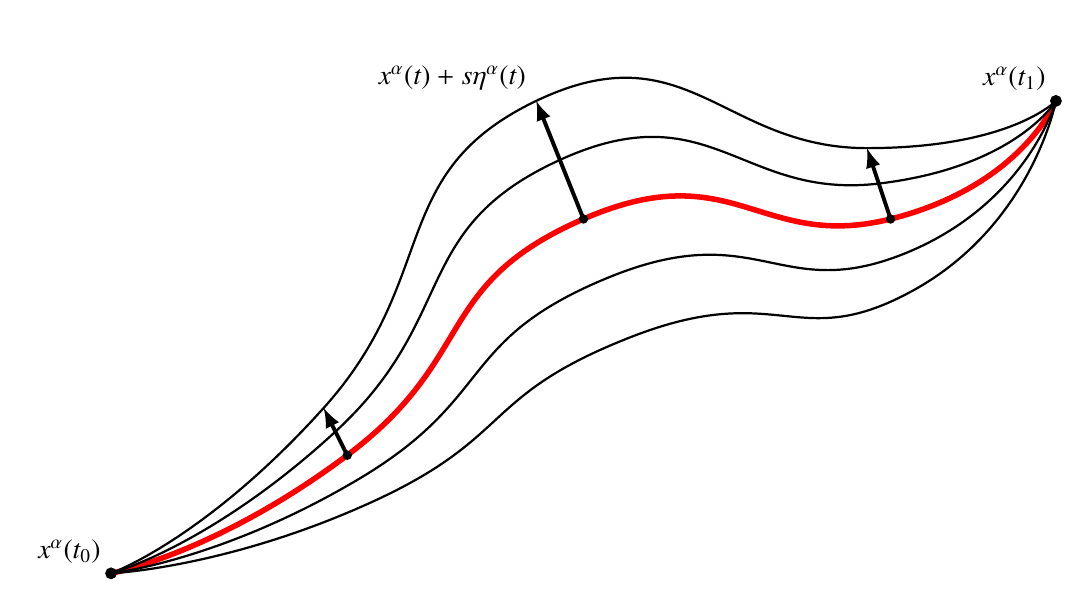
\begin{tikzpicture}[>=latex, thick, scale = 3, fixed point arithmetic]

\coordinate (O) at (0,0);

\draw [red,line width=0.7mm] plot [smooth, tension=1] coordinates {
	(0,0) (1,0.5) (2,1.5) (3.3,1.5) (4,2)
};

\draw [black] plot [smooth, tension=1] coordinates {
	(0,0) (1-0.1,0.5+0.2) (2-0.2,1.5+0.5) (3.3-0.1,1.5+0.3) (4,2)
};
\draw [black] plot [smooth, tension=1] coordinates {
	(0,0) (1-0.05,0.5+0.1) (2-0.1,1.5+0.25) (3.3-0.05,1.5+0.15) (4,2)
};
\draw [black] plot [smooth, tension=1] coordinates {
	(0,0) (1+0.1,0.5-0.2) (2+0.2,1.5-0.5) (3.3+0.1,1.5-0.3) (4,2)
};
\draw [black] plot [smooth, tension=1] coordinates {
	(0,0) (1+0.05,0.5-0.1) (2+0.1,1.5-0.25) (3.3+0.05,1.5-0.15) (4,2)
};

\draw[fill=black] (0,0) circle[radius=0.2mm,fill]{};
\draw[fill=black] (4,2) circle[radius=0.2mm,fill]{};

\draw[->,line width=0.5mm] (1,0.5) -- (1-0.1,0.5+0.2);
\draw[->,line width=0.5mm] (2,1.5)--(2-0.2,1.5 + 0.5);
\draw[->,line width=0.5mm] (3.3,1.5)--(3.3-0.1,1.5+0.3);

\draw[fill=black] (1,0.5) circle[radius=0.15mm];
\draw[fill=black] (3.3,1.5) circle[radius=0.15mm];
\draw[fill=black] (2,1.5) circle[radius=0.15mm];

\draw (0,0) node[above left] {$x^\alpha(t_0)$};
\draw (4,2) node[above left] {$x^\alpha(t_1)$};
\draw (2-0.2,1.5+0.5) node[above left] {$x^\alpha(t) + s\eta^\alpha(t)$};

\end{tikzpicture}
\end{document}

